\documentclass[notitlepage,letterpaper,pdftex,12pt,final]{article}
%\documentclass[notitlepage,letterpaper,pdftex,12pt,draft]{article}
% article < report < book ; preable material follows
%
% This file is mostly boilerplate that you can copy and tweak.
% The true material is in included files.  ../common should hold
% things that more than one document might need.  The Makefiles
% should likewise be mostly boilerplate with minor tweaks.
%

% (un)comment to (see)hide full paths to files actually used
% however, you'll need to override the TEXOPT= setting to batchmode
% made in the Makefile.
\listfiles

\addtolength\textwidth{1.7in}
\addtolength\oddsidemargin{-0.95in}
\addtolength\evensidemargin{-0.95in}
\addtolength\marginparwidth{-0.95in}
\typeout{textwidth is \the\textwidth}

% useful to block out portions of text
\usepackage{ifthen}
% to allow defining our own colors
\usepackage[dvipsnames]{xcolor}
% makes hyperlinks work
\usepackage{hyperref}
\hypersetup{colorlinks=true,linkcolor=darkblue,citecolor=darkgreen}
% for figures; insert [draft] before {...} not to see imgs
\usepackage{graphicx}
\graphicspath{ {../common/uml-diagrams} }
% for small figures surrounded by text
\usepackage{wrapfig}
% for control over headers and footers
\usepackage{fancyhdr}
\pagestyle{fancy}
\fancyhf{}
% for handling acronyms
\usepackage[printonlyused]{acronym}

% for bibliographies if needed
\usepackage[utf8]{inputenc}
\usepackage[english]{babel}
\usepackage[backend=bibtex,style=numeric,sorting=none]{biblatex}
\addbibresource{hops.bib}
%\usepackage{natbib}
% Use the appendix package.
\usepackage{appendix}
% context-sensitive quotes
\usepackage{csquotes}
% underline for emphasis: \uline etc
\usepackage{ulem}
% for generating outlines
\usepackage{outlines}
\usepackage{enumitem}

% for bold math
\usepackage{bm}
% for serious math which we may have in a few places (eventually)
\usepackage{amsmath}
% equations include section number
\numberwithin{equation}{section}

% for marginal notations concerning geodesy
\usepackage{marginnote}

% to go back to default after \ragged commmands
\usepackage{ragged2e}

% see common/shortcuts.tex for what is defined in this file
%
% a file of commands to save typing
%

% commonly used things
\newcommand{\eg}{\textit{e.g.}}
\newcommand{\EG}{\textit{E.g.}}
\newcommand{\ie}{\textit{i.e.}}
\newcommand{\IE}{\textit{I.e.}}
\newcommand{\etc}{\textit{\&c.}}
\newcommand{\Sec}{Section}
\newcommand{\Fig}{Figure}
\newcommand{\Tab}{Table}
\newcommand{\App}{Appendix}

% for a work in progress:
\newcommand{\FIX}[1][fixme]{{\color{red}#1}}
\newcommand{\TBC}{{\color{red}TBC}}
\newcommand{\TBD}{{\color{red}TBD}}
\newcommand{\TBR}{{\color{red}TBR}}
\newcommand{\FIXME}[1][]{{\color{red}FIXME -- #1}}

% specific to this project
\newcommand{\MHO}{MIT-HOPS}
\newcommand{\HOPS}{HOPS}

% standard colors
\definecolor{darkblue}{rgb}{0,0,.5}
\definecolor{darkgreen}{rgb}{0,.5,0}
\definecolor{darkred}{rgb}{.5,0,0}
\definecolor{violet}{rgb}{.4,0.,.7}

% for coping with geodetic things
\newboolean{geos}
\setboolean{geos}{true}% or false to hide geodetic marginal notations
%
\definecolor{boxfrcolor}{rgb}{.50,.20,.00}
\definecolor{boxbgcolor}{rgb}{0.9,.98,.98}
\definecolor{boxfgcolor}{rgb}{0.4,0.0,0.0}
% \geomargin{footnote comment}
% \geomargin[{\color{..}box note}]{footnote comment}
\newcommand{\geobox}[1]%
{{\parbox{10mm}{\small\textit{\fcolorbox{boxfrcolor}{boxbgcolor}{#1}}}}}
\newcommand{\geomargin}[2][{\color{boxfgcolor}geodesy}]%
{\ifthenelse{\boolean{geos}}{% if:
\marginnote{\protect\geobox{#1}}\footnote{#2}}{% else: show nothing
}}

% for itemizing requirements
\newcounter{req}
\newcommand{\reqid}[1]{\item[\refstepcounter{req}#1-\thereq]}

%
% eof
%

\setboolean{geos}{false}% or false to hide geodetic marginal notations

% control options
\newboolean{skipappendix}
\setboolean{skipappendix}{false}

% at some point this gets frozen
\newcommand{\recdate}{\today}

\begin{document}
\DeclareGraphicsExtensions{.png, .jpg, .pdf}
% best to put figures in subdirs
%\graphicspath{{figs/}{scans/}}

% for subsequent pages
\setlength\headheight{15pt}
\fancyhead[L]{HOPS}
\fancyhead[C]{}
\fancyhead[R]{Requirements}
\fancyfoot[R]{Page \thepage\ of\ \pageref{page:LastPage}}
\fancyfoot[L]{\recdate}

\title{ngEHT Requirements for a new HOPS}

\author{%
\LARGE John Barrett, Geoff Crew, Dan Hoak and Violet Pfeiffer \\
\Large MIT Haystack Observatory}
\date{Version 1.0, \recdate}
\maketitle
\normalsize

\renewcommand\abstractname{\large Executive Summary}
\abstract{
This document spells out the requirements for the planned re-work of HOPS.
With a defined set of requirements (\Sec~\ref{sec:testable}),
we can ensure that the new architecture
and implementation supports the needs.  And by the conclusion of the project
a collection of test reports matching results to requirements may be presented.

Note that there is an implicit desire to end up with a suite of software that
not only meets the stated needs, but which also is easier to maintain, and more
extensible for the future.  While we might state these desires as requirements,
it is not possible to test against them, and thus these do not formally appear 
in this document, and are discussed elsewhere.
}

% N.B.: NASA document describing preferred language for enumerating requirements:
% https://www.nasa.gov/seh/appendix-c-how-to-write-a-good-requirement


% \begingroup . . . \endgroup can be used to keep things together
% and/or an explicit page break and/or adjust spacing as needed so
% it looks presentable.  Uncomment the sections you need.
%\begingroup
%\renewcommand\contentsname{Contents}
%\renewcommand\listfigurename{Figures}
%\renewcommand\listtablename{Tables}
%\vspace{24pt}\hrule

\pagebreak
\tableofcontents

%\vspace{24pt}\hrule
%\pagebreak
%\listoffigures
%\vspace{24pt}\hrule
%\listoftables
%\vspace{24pt}\hrule
%\endgroup

% it is sometimes cleaner to start sections on new pages in a longer
% document--then changes to each section don't repage everything.

% break document into appropriate portions

\pagebreak
%
% introductory thoughts
%

\section{Introduction}
\label{sec:intro}

The \ac{EHT} has launched a \ac{MSRI} project which looks to develop
the technologies needed for a second-generation \acs{EHT}. 
A significant component of the telescope is the software needed to 
properly operate, reduce and analyze the data taken by the member telescopes.
This document defines the requirements for the refactoring of the \ac{HOPS} in 
concert with the \acs{MSRI} proposal. 

The next generation \acs{EHT} is planned to include up to 30 stations and 
435 baselines, with wider bandwidth (128 Gbps has been mentioned---meaning 
four dual-polarization, 4 GHz bands) \TBR{}.  Support for greater bit depth is also of 
interest should recording media be available.  The refactoring
of \ac{HOPS} shall support the full analysis of ngEHT data within these limits,
and will be made smarter, more automatic, more robust, and easier to use.

%Furthermore, the \acs{EHT} may elect to operate with a more frequent observing cadence. 

For the needs of the \acs{EHT} Campaigns of 2017 it was decided to augment
the existing HOPS package with some Python-based packages in order to
create a pipeline for the initial reduction of data. The new \ac{HOPS} shall
support independent analyses, using Python or other languages, through
accessible data formats (e.g. HDF5, JSON, XML, or similar), interactive tools, and 
conversion to human-readable ASCII files. The current plotting functionality,
provided by PGPLOT, shall be replaced by Python/Matplotlib.

%In this continued development of HOPS, we shall assume
%that HOPS alone must be capable of the full analysis; but we should also
%be mindful that options to move the data to \ac{AIPS} or \ac{CASA} must at some
%level exist.

The primary development language will be C/C++, with a Python scripting layer
to provide ease of use. Version control shall be provided by the MIT-hosted github.

Finally, all functionality of the current \acs{HOPS} shall be maintained, with
backward-compatibility for old data formats. There shall be extensive use of regression
tests and demonstrated reproducibility of prior results.

This document is intended to be one in a series, with other documents describing:
\begin{itemize}
\item Specifications and architectural design
\item Coverage and test plan
\item The development plan
\item The user manual
\item Requirements specific to geodesy
\end{itemize}




%This section enumerates specific requirements that we plan to meet by test.
%Note that there are many untestable ``desires'' or ``goals''; these are
%discussed in then next section (\Sec~\ref{sec:desires}).  Consequently,
%potential tests that address such things do not appear in this section.
%These issues are more fully addressed in the design document (\cite{design}).
%
%The itemization and description of thest tests are partitioned into
%subsections according to how they are likely to be executed.
%The first section deals with short automated tests
%(\Sec~\ref{sec:auto}, \ie~these that that may be executed
%in a nightly build), software tests that may be run at specific
%juctions (\Sec~\ref{sec:regress}, \ie~regression tests),
%and tests that are procedural, requiring human interaction
%(\Sec~\ref{sec:procedure}, \ie~\ac{GUI} tests).%
%\geomargin{In addition to these requirements, there are a few additional
%geodetic requirements which are captured outside the ngEHT effort.}
%Details of the testing process are to be found in the coverage
%and testing document (\cite{cover}).
%
%\acs{HOPS} is currently in the version 3.x series; the new code will
%begin with the 4.x series, and to distinguish the two flavors, (in code
%and otherwise) we shall use \acs{MHO} to specifically refer to the latter.
%
%The requirements in this document are numbered with a prefix
%according to the type of test that may be employed:
%A for automated tests, S for software testable, P for procedural.
%The desire and goals are prefixed with D for desire and
%F for future-proofing.
%
%\subsection{General Requirements}
%\label{sec:generalreq}
%
%It is anticipated that each of these tests will be captured by a
%``check'' (shell or Python) script (such as currently supported in
%the autotools or created to more fully ensure safe development).
%Existing unit tests within \ac{HOPS} will be ported into the
%new \ac{MHO} code set.



%
% eof
%


\pagebreak
%
% the meat of the thing
%
% a counter for consecutive numbering and \reqid are defined in shortcuts.
%

\section{Requirements}
\label{sec:testable}

%This section enumerates specific requirements that we plan to meet via explicit
%tests.
%Some
%Note that there are many untestable ``desires'' or ``goals''; these are
%discussed in then next section (\Sec~\ref{sec:desires}).  Consequently,
%potential tests that address such things do not appear in this section.
%These issues are more fully addressed in the design document (\cite{design}).
%
%Requirements shall generally be paired with explicit demonstrations that they
%have been met.
%


%The requirements defined in this section
%are partitioned into subsections according to how they are likely to be executed.
%The first section deals with short automated tests
%(\Sec~\ref{sec:auto}, \ie~these that that may be executed
%in a nightly build), software tests that may be run at specific
%juctions (\Sec~\ref{sec:regress}, \ie~regression tests),
%and tests that are procedural, requiring human interaction
%(\Sec~\ref{sec:procedure}, \ie~\ac{GUI} tests).%
%\geomargin{In addition to these requirements, there are a few additional
%geodetic requirements which are captured outside the ngEHT effort.}
%Details of the testing process are to be found in the coverage
%and testing document (\cite{cover}).

The requirements defined in this section are loosely organized by functionality.
Requirements are numbered with a prefix according to
the type of test that will be used to validate them.  These prefixes are:
%%% EDIT: \item[A,] etc. to avoid the awkward-looking lonely comma
\begin{description}
[align=left, labelwidth=0.0cm, leftmargin=1cm]
\item[A,] for automated tests. These are requirements
that shall be validated with a ``check'' script (in shell, Python, or similar).
These scripts can be executed during installation steps to verify the
installation was successful,
or in a nightly build to verify that daily updates have not broken any
functionality. Existing tests within HOPS3 will be ported into the new
HOPS4 code set.

\item[S,] for software-testable. These are more complicated tests such as
regression tests that may be run at specific points in development. It is
anticipated that each of these tests will be implemented by a script, and a report provided.

\item[P,] for procedural tests that require human interpretation (\eg
validating the display mechanics of a figure). These tests shall have
explicit instructions for the user and the results shall be recorded.

\item[D,] for desires. These are general design goals for which testing reports are not required.

%\item[F,] for future-proofing guidelines to ensure HOPS4 is useful beyond
%the immediate horizon. For every required package (beyond the historically,
%generally available GNU/Linux packages) the code should be structured
%so that it is relatively straightforward to port to a new package with
%similar functionality. Again, no formal test report for these shall be made.

\end{description}

Details of the testing process will be made available in the coverage
and testing document \cite{cover}.
%%% EDIT: my preference here would be to site the document as
%%% EDIT: being ``in preparation''.  We know the title and authors.

%\FIX[Note: many of these requirements were imported from existing check
%scripts and need explicit definitions. The tests need to be reworded into 
%``requirement'' form. The requirements should have ``rationale'', ``explanation'',
%``comment'' or some other clarification as appropriate]




%\subsection{Automated Testable Requirements}
%\label{sec:auto}
%
%The following are essential design requirements that shall be validated with a
%``check'' script (shell, Python, or similar). The current \acs{HOPS}
%incorporates many scripts of this sort, which are used during the compile and
%installation steps to verify the installation was successful, and during nightly
%builds to verify that daily updates to the code base have not broken any
%functionality. Existing unit tests within \ac{HOPS} will be ported into the new
%\ac{MHO} code set.
%
%In addition to check scripts, unit tests shall be used for all code fragements,
%and shall cover all code.



%%%%%%%%%%%%%%%%%%%%%%%%%%%%%%%%%%%%

\subsection{General Requirements}
\label{sec:genreq}

The following requirements describe essential design features.

\begin{description}

\reqid{S} HOPS4 shall provide effectively equivalent results for any output that HOPS3 was capable of producing.
\reqex{A sufficient set of historical DiFX output has been captured and HOPS4 results will 
be periodically compared to HOPS3 results on observables that HOPS3 supports to ensure consistency.}

\reqid{A} HOPS4 shall have no practical limit on the number of stations,
baselines, channels, or accumulation periods other than which is imposed by the
memory limitations of the computer hardware on which it is run.

%%% EDIT: it think it is useful to leave these red

\reqid{A} HOPS4 shall support at least \FIX[30] stations and 435 baselines.
  \reqex[input required]{HOPS4 requires an upper bound merely to verify that
    it supports ``more than enough''}

\reqid{A} HOPS4 shall support at least \FIX[128] channels and should not impose a
 limit on the number of channels.
  \reqex[input required]{HOPS4 requires an upper bound merely to implement
    with some sensible channel labeling scheme and verify that the requirement is satisfied.}
    %\footnote{using \acs{Unicode} for channel labels would certainly
    %be unbounded, but might be challenging for some to type. However,
    %there is no real need to limit channel labels to a single-character.}

\reqid{A} HOPS4 shall support a (raw station data) bit depth of \FIX[2] bits.
  \reqex[input required]{Support for 1-bit is available in HOPS3,
    and hooks for other bit depths will be provided, but the code for other
    depths will require development in order to ensure proper normalization
and treatment of noise statistics, etc.}

\reqid{A} Every library (C/C++) or module (python) shall have a corresponding
test suite to verify expected functionality, this may include but is not limited
to unit tests (for individual classes/functions) with the appropriate test
cases to be determined.


\end{description}

The existing package has a number of dependencies which are becoming
a challenge to maintain---\acs{PGPLOT} is such an example.  Ideally
HOPS4 should be installable and usable without any dependencies.
(However, we shall not require that the software provide complete functionality
on a computer lacking such optional dependencies.) The build machinery should test
for the presence of these packages and make appropriate accommodation for
the Linux distribution. Note that we will only support three major distributions,
Debian/Ubuntu, Fedora, and NixOS. Testing will be done frequently for only these
three distributions. There are no plans to officially support other distributions,
Mac OSX, or Windows.

\begin{description}

\reqid{P} HOPS4 shall operate without loss of functionality in the absence of
FFTW3, and/or GSL, with the understanding that performance (runtime) might be
affected. 
\reqex{For example FFT calls should be wrapped so that other
packages or native code may be used instead.}

\reqid{P} \acs{PGPLOT} shall not be required for basic functionality (\eg
fringe-fitting),
though it may be optionally supported for some plotting/display options.
\reqex{The \acs{PGPLOT} package has been out of maintenance for a long time,
and any replacement package could follow the same fate. Thus all plotting package calls need to be 
managed within an optional plugin which leaves core functionality unaffected by 
its presence. At a minimum, plotting functionality similar to the current fringe-plots
can be constructed as a set of independent Python tools.}

\end{description}

%The following existing tests currently exist in \ac{HOPS}
%and can be ported to pass in \ac{MHO} as well.
%\FIXME[This list is not currently well-ordered.]
% find . -name Makefile.am -print \
% -exec sed '/TESTS[^_].*=/,/^$/!d' {} \; -print | sed 's/^/% /' |
% grep -v PROGRAM



%%%%%%%%%%%%%%%%%%%%%%%%%%%%%%%%%%%%

\subsection{File I/O and Supported File Types}
\label{sec:ioreq}

\begin{description}

\reqid{A} HOPS4 shall support input from the DiFX \cite{deller2007difx,deller2011difx} correlator (in Swinburne format).

% ./vex2xml/Makefile.am
\reqid{A} every application should provide
    \verb+--help+ and \verb+--version+ responses (with zero exit status)
    to behave as conventional \acs{GNU/Linux} applications.
  \reqex{Command-line arguments should be implemented with a
    standard argument parsing library, and should respond helpfully
    on bad command-line syntax.}

\reqid{A} HOPS4 shall support input from \acs{VEX} version 1.5.\footnote{\acs{VEX} 1.5
is the only extant working file format for VLBI experiment description, however, there does
exist a VEX 2.0 specification which is not currently in active use but may be adopted at any time.}


\reqid{A} All plotting tools provided in HOPS4 shall have the ability to save the image to 
a standard graphics format.

% ./sub/dfio/Makefile.am
%\reqid{A} If the non-compressed form of the \acs{Mk4} fringe file will be
%supported, we require that the results of fourfit (captured in the fringe plot)
%be identical to results from the compressed version.
%\reqex{\texttt{test\_compress} is an existing test of the \acs{PostScript}
%compression used in the \acs{Mk4} fringe file format. \FIXME[This requirement will likely
%disappear - we will save plots directly in PDF format, and save data in a
%file. No more parsing postscript files for fringe results!]}

\reqid{D} All new native data types (to be detailed in the specification document)
shall be stored \acs{littleendian}.

\reqid{D} HOPS4 shall provide an application to support export of native
data types to a \TBD~archival format (\eg~HDF5).

\reqid{D} HOPS4 shall incorporate a C-library to interface with the legacy 
\acs{Mk4} data types (stored \acs{bigendian}) in their current form for 
testing purposes, and in order to access archived data. 
%HOPS4 
%will not, however, be required to support any new functionality.

\end{description}



%%%%%%%%%%%%%%%%%%%%%%%%%%%%%%%%%%%%

\subsection{A-tools}
\label{sec:areq}

The following requirements are related to the ``A-suite'' tools \acs{alist}, \acs{aedit},
and \acs{adump}.  The command-line interface for these tools shall be wrapped
in Python in HOPS4 and shall support alist file version 6\footnote{Version 6 is the standard for the \ac{EHT}, and a version 7 format seems
sensible but not yet required.  If in detailing the specifications
a version 7 (or 8, \etc) emerges, these requirements transfer
to the those version(s) as well.]}.

%%% EDIT: replaced:
%%% 5 \& 6 \footnote{%
%%% If there is an \acs{A-list} version 7, these shall apply to version 7 as well.
%%% A discussion of a TDB version 7 \acs{alist} shall be included in the
%%%  specifications document.}.

%\vspace{12pt} \EDIT[DROPPING ALL MENTION of 5 and geodesy.]


\begin{description}

\reqid{A} The \acs{alist} program shall generate valid \acs{A-list} files in 
version 6.

%\reqex{\texttt{chk\_alist.sh} currently does this for versions 5 and 6.}

%\reqid{A} the \acs{alist} program shall provide a new ASCII
% A-list format (version 7) that will allow the data columns will be user-defined.

\reqid{A} The \acs{adump} program shall provide valid ASCII text representations 
of columns of data from an \acs{A-list} of version 6.
%\reqex{\texttt{chk\_adump.sh} currently does this for versions 5 and 6.}

\reqid{A} The \acs{aedit} program shall process version 6 \acs{A-list} 
files with respect to flagging, selecting, summarizing and generating a new 
output \acs{A-list}.
%\reqex{the \texttt{chk\_aedit.sh} currently makes a pass through many of these}

%\reqid{A} the \acs{Python}ic replacement module for these three current
%    applications (alist, aedit, adump), must fulfill the same requirements.

% ./data/ae_testdata/Makefile.am

%%% EDIT: drop this here:
%%% \reqid{A} HOPS4 shall maintain the performance of \acs{aedit} version 5 (for 
%%% geodesy) and 6 (for EHT).
%%%


%\reqex{Currently, \texttt{chk\_fsumm.sh} performs such a test with captured 
%\acs{A-list} data.}

%\reqid{S} \acs{aedit} experiment summary plot test.  This requires a
%    human to verify that the summary is displayed, and that clicking
%    on a scan-baseline-pol point produces the appropriate fringe plot.
%\reqex{\FIXME[need to elaborate on the requirement that is being tested]}
%
%\reqid{S} \acs{aedit} quantity with time display plot.  This requires
%    a human to verify that the desired data are shown, and that it
%    is possible to flag (discard) points.
%\reqex{\FIXME[need to elaborate on the requirement that is being tested]}
%
%\reqid{D} Expand the functionality of \acs{alist} to allow for more data
%
%    analysis/visualization options.
%  \reqex{\acs{Python} seems a likely solution, also Looker or Tableau.}
%
%\reqid{D} Refactor how alist files are handled to make one line
%    summaries of every fringe plot but do it in Python.

%\reqid{D} Refactor alist, aedit, and fourfit to be compatible with \ac{HOPS}.
%\reqex{\FIXME[need to elaborate on this desire]}

%\reqid{A} \acs{aedit} backwards compatibility on version 5, 6 and
%    any version \TBD~7 shall be maintained.

%\reqid{A} \FIXME[what does this test test, actually]
%    (\texttt{test\_mk4fringe} a test related to the uncompress
%    or compressed storage of \acs{Mk4} fringe files)
%
%\reqid{A} \FIXME[what does this test]
%    (\texttt{chk\_baselines.sh})

\end{description}


%%%%%%%%%%%%%%%%%%%%%%%%%%%%%%%%%%%%

\subsection{Post Processing and Fringe Plots}
\label{sec:postprocreq}
%This section will outline to the components of HOPS that are affected by the HOPS refactoring effort.

The following requirements describe wrappers and tools in HOPS3 for 
post-processing and examination of the fringe results. They shall be
maintained in HOPS4.

%\FIXME[Same as above: re-write these as specific requirements, move check script details to the
%coverage and testing document.]

\begin{description}
% ./postproc/fourmer/Makefile.am
\reqid{A} HOPS4 shall maintain the \acs{fourmer} tool, which shall properly 
relabel channels when it combines two sub-bands.
%\reqex{This is currently performed by \texttt{test\_new\_chan\_id}.}

\reqid{A} The \acs{fringex} program shall retain existing functionality to rotate
fringes with respect to fourfit fringe solutions.
%\reqex{The \texttt{chk\_fringex.sh} exists to verify this in HOPS3.}

\reqid{A} The ``average'' capability, implemented by \acs{average} used in 
concert with \acs{fringex} to subdivide explore and average fringes, shall be 
preserved with equivalent functionality.
%\reqex{The \texttt{chk\_average.sh} program tests this for the existing 
%\acs{average} application, but the piping mechanism is cumbersome and should be
%re-implemented in a more easily used (and likely more efficient) C/C++ or 
%\acs{Python} application.}

\reqid{A} The functionality of the program \acs{cofit} shall be preserved.
%\reqex{\texttt{chk\_cofit.sh} currently verifies this.}

%%% ``there''
\reqid{A} The current functionality of the program \acs{search} shall be 
preserved.
%\reqex{\texttt{chk\_search.sh} currently verifies this by performing a search on
%a captive data set.}

%%% EDIT: duplicate
%%% \reqid{A} There shall continue to be a functional \acs{fourmer} tool to assemble
%%% separately correlated frequency sub-bands.
%\reqex{\texttt{chk\_fourmer.sh} currently does this for a captive two 512-MHz 
%bands. We will need to build and maintain a test to cover an extension to 
%current \acs{EHT} 2-GHz bands.}

\reqid{A} The ability to explore fringes (as is currently done with the 
combination of \acs{fringex}, \acs{average} and search must be preserved. 
HOPS4 shall support \acs{Python} scripting to aid the user in searching 
fringe space.
%\reqex{The \texttt{chk\_frmrsrch.sh} script executes such a case.}

\reqid{P} It should be possible to make 2D plots of the type currently possible 
within \texttt{\acs{aedit}} of HOPS3.
\reqex{These are plots such as \acs{SNR} with time broken out by baseline with 
separate symbols per target. It is not currently possible, but should be possible 
to combine several baselines into a composite plot.}

\reqid{P} It should be possible to make 3D visualization plots.
\reqex{\acs{search} makes contour plots, but a 3D visualization of amplitude 
with delay and delay-rate would be useful.}

\reqid{P} HOPS4 shall implement interactive visualization tools in for \acs{fourfit}.
\reqex{The HOPS3 version of \acs{fourfit} provides a fixed fringe summary
plot. HOPS4 should have an interactive plotting capability to enable zooming
and viewing fourfit results with an expanded scale.}

\reqid{D} Replace the existing \acs{fourfit} control file with a 
\acs{Python}-based control file. Currently existing functionality shall be be 
preserved. 
\reqex{The existing control file should continue to be supported, but new 
functionality might only exist in the HOPS4 toolset.}


\end{description}


%%%%%%%%%%%%%%%%%%%%%%%%%%%%%%%%%%%%

\subsection{Miscellaneous Requirements}
\label{sec:miscreq}

\begin{description}
    
\reqid{A} It shall be possible to automatically discard correlator 
\acs{AP} (integrations) with small weights.
\reqex{When data are poorly recorded, the correlation product is the result 
of less data than it should be, leading to incorrect results. This is currently done in HOPS3 provided \acs{DiFX} properly notices the loss.}
%The HOPS3 script 
%\texttt{chk\_min\_weight.sh} currently tests this capability. In addition, 
%user-supplied ad-hoc flagging capability is tested by \texttt{chk\_flagging.sh}.}

\reqid{A} HOPS4 shall have the ability to flag data based on a user-supplied 
list (\eg~of frequency intervals with time in some flag file).
\reqex{This is needed especially when \acs{RFI} or calibration tones signals 
are present.}%  In HOPS3 \texttt{chk\_notches.sh} verifies this.}

\reqid{A} Every data type written to disk in HOPS4 shall be convertable to 
form that is amenable to human examination (e.g. ASCII or CSV), as is done in HOPS3 by the 
\texttt{\acs{CorAsc2}} program.
%\reqex{For the HOPS3 \acs{fourfit} program, this is verified by 
%\texttt{chk\_ff\_dump.sh}; for \acs{A-list} data, this is provided by \acs{adump},
%or some combination of awk, sed and grep.}

\reqid{A} HOPS4 shall implement an algorithm for solving for station-based 
quantities from baseline-based quantities as a global fringe fitter.
\reqex{This is new for HOPS.}

% I (DH) think this refers to converting delays from the basis of 
% baselines (between two stations) to the basis of individual stations,
% i.e. using sets of three (triangular) baselines to calculate the 
% delays at each station.

\reqid{A} The HOPS4 \acs{fourfit} shall have the ability to apply complex 
bandpass correction.
\reqex{This is a new capability that might well be prototyped in the existing 
HOPS3 package. Here ``complex'' refers to both amplitude and phase variation 
of the receiver frequency response. HOPS3 already has rather 
sophisticated phase calibration handling. \geomargin{the \acs{EHT} does 
not use tone generators, so most of that is only useful for geodetic systems 
which do} The ``manual'' phase calibrations already handle the phase 
variation from between \acsp{channel}.  HOPS3 has no amplitude adjustment 
capability.  The desire is for a more flexible arrangment that is not limited
by channel boundaries.}

\reqid{A} HOPS4 shall provide a method to solve for complex bandpass corrections.
\reqex{This method should accept some set of scans and stations and solve, 
possibly using an \acs{LSF} method, for per-station bandpass solutions}

\reqid{A} Python wrappers for the new HOPS4 data objects shall be provided.
\reqex{The existing wrappers for the \acs{Mk4} data types in HOPS3 do not 
need to be preserved, but it is a capability worth preserving.}


\reqid{D} The HOPS4 suite must provide mechanisms to preserve the correlator 
output data.
\reqex{A \acs{PERL} script, \texttt{hops\_data\_links.pl}, exists to manage 
symbolic links to analysis files in a working directory separate from the original 
correlator output directory.}
%A script, \texttt{chk\_hdlinks.sh}, verified this capability 
%in HOPS3, and a similar mechanism should be provided in HOPS4.}

\reqid{D} HOPS4 should preserve the the Single Band Delay, Multi Band Delay 
and Delay Rate search algorithm in its current form.
\reqex{Our desire is to make the algorithm modular, such that the user may (de)select search
dimensions. For example the current loop in in \acs{fourfit} includes a loop over \acs{TEC},
which is not needed at \acs{EHT} frequencies and could be ignored in \acs{EHT} analysis. 
Similarly, for spectral line data the multi-band delay is not meaningful.
The revised implementation should make it easier to develop and
introduce new algorithms.}.
%The current loop in \acs{fourfit} includes a loop over \acs{TEC}
%(which is not needed at \acs{EHT} frequencies), which makes 4 loops.  For spectral line data 
%\acs{MBD} is impossible, so there are two loops too many.



\reqid{D} Benchmarking and performance analysis should be augmented with 
a more sophisticated tools.
\reqex{The existing HOPS package supports a \texttt{account} library that does 
rudimentary profiling.  Introducing \texttt{gprof} into some specific build tests, 
should be straightforward and help to optimize fringing.}

\reqid{D} HOPS4 should support spectral-line VLBI.
\reqex{The existing HOPS code assumes a continuum.}

\reqid{D} HOPS4 should support pulsar folding with a user specified period or
ephemeris file with blanking.
%\reqex{This may be descoped.}

\reqid{D} HOPS4 should enable multi-threading or multi-processing for batch jobs.
\reqex{Parallelization is a strong desire, but the exact details of the 
implementation (particularly the requirements of threads vs processes) need to 
be carefully designed.}


\end{description}



%%%%%%%%%%%%%%%%%%%%%%%%%%%%%%%%%%%%




%\subsection{Procedure-Testable Requirements}
%\label{sec:procedure}

%This section includes items that may be directly verified in a quasi-automated
%fashion which may involve a human.  That is, there will be a procedure for the
%human to execute with a documented report to be generated.






%
% apparently the description environment breaks the math here, so
% relative math adjustments will be needed if these are reordered
%
%\newsavebox{\xpgplot}
%  \addtocounter{req}{1}
%  \sbox{\xpgplot}{\textbf{{P-\thereq}}}
%\newsavebox{\xfftwthree}
%  \addtocounter{req}{1}
%  \sbox{\xfftwthree}{\textbf{{P-\thereq}}}
%\addtocounter{req}{-2}
%

%\FIXME[more of these?]

%\section{General (not directly testable) Desires}
%\label{sec:desires}

%\subsection{Current Desires}
%\label{sec:currentdesires}
%
%This section covers items that are verifiable by inspection (or analysis
%or discussion).  It is subdivided into a section on goals of the current
%project which we expect to reach by the end of the project, and a section
%on future-proofing.

%\begin{description}
%\reqid{D} Everything currently possible in \ac{HOPS} should remain
%    possible in \ac{MHO}.
%  \reqex{The existing tests mostly cover this.}
%\reqid{D} \ac{MHO} should be easier to use than \ac{HOPS}.
%  \reqex{The decision to add a \acs{Python} scripting layer (similar
%    to \acs{CASA} addresses this.}

%\reqid{D} Rename the Mk4 data type number series.
%\reqid{D} Refactor all existing algorithms in to new Python libraries
%    that run C or C++ code under the hood.

%\end{description}





%
% eof
%


\pagebreak
\addtocounter{section}{1}
\renewcommand{\refname}{\thesection. References}
\addcontentsline{toc}{section}{\thesection. References}
\bibstyle{plainurl}
\printbibliography
\label{sec:references}

% if skipappendix-is-true then (nothing) else typeset Appendices
\ifthenelse{\boolean{skipappendix}}{}{%
\appendix

%\pagebreak
%%
% the meat of the thing
%
\section{What was promised at HILO}
\label{sec:hilo}

This appendix captures what was presented at the Hilo
\ac{EHT} meeting (Dec. 2019) in a software session intended to
capture feedback on the plan.  The discussion
did not provide any clear guidance to adjust our plans.

\newcommand{\sbitem}{\hfill\break\hspace{2mm}$\diamond$\ }

\subsection{slide 2}
\begin{itemize}
\item \ac{HOPS} performed adequately for 2017 data reduction
\sbitem consistency with \ac{AIPS} and \ac{CASA} was established
\sbitem the \ac{HOPS}-based pipeline was adopted for production
work\footnote{%
after validation against the alternatives using \ac{AIPS} and \ac{CASA}.
We consider it still highly valuable to update \ac{HOPS}, and indeed, it
makes sense to enable interoperability with \ac{CASA}---however, that is
outside of our scope.}
\item The \ac{ngEHT} funding via \ac{MSRI}-I calls for updates to HOPS:
\sbitem 4 years of development to become “shovel ready”o
\sbitem N stations more than doubles (\eg to 20-30)
\sbitem Bandwidth quadruples at some sites (\eg 8 GHz)
\sbitem Simultaneous 230 / 345 \ac{GHz} observing perhaps
\sbitem Anything else that gets decided in then next 4 years
\end{itemize}

\subsection{slide 3}
\begin{itemize}
\item We’ve (almost) come to the end of what can be fixed with “bandaids”
\item Maximum \# of channels is 64 and that’s hard to fix (a-zA-Z0-9\%\$)
\item No full complex bandpass corrections (only per-channel phase+delay)
\item single-baselines are both a virtue and a problem:
\sbitem \ac{HOPS} finds more fringes than \ac{AIPS} or \ac{CASA}.
\sbitem station-based phases and delays are not readily accessible
\item \ac{fourfit} is a one-shot process; multi-step processing not supported
\item User interface is a challenge:
\sbitem control file syntax is a bit arcane
\sbitem all you get is one \ac{fourfit} plot that either works or is garbage
\end{itemize}

\subsection{slide 3}
\begin{itemize}
\item \ac{HOPS} code has 30+ years of history in it
\sbitem was coded in \ac{C}, but reads like the \ac{Fortran} it was ported from
\sbitem not modular except for a few of the i/o libraries
\sbitem was written for hardware correlators
\sbitem was written for computers that no longer exist
\sbitem little endianism won out over big endianism (apparently)
\sbitem was (successfully) successfully adapted to \ac{DiFX}
(but not \eg \ac{SFXC})
\item Plotting and results are not independently generated
\sbitem amplitude and \ac{SNR} come as side-effects of what you plotted
\sbitem \ac{PGPLOT} is maybe ok today, but not really supported anymore
\end{itemize}

\subsection{slide 4}
\begin{itemize}
\item Global fringe solutions (and station based-quantities)
\item Complex bandpass
\item A more human-friendly interface (\eg \ac{Python} as \ac{CASA} does)
\item Allow distributed computing and/or parallelization (threads, OpenMPI)
\item Insert hooks to allow plug-in modules for customizations as needed
\item Allow a strategy for iterative calibration and fringing
\item Improved data formats (internal in-memory as well as disk storage)
\item Enable better exchange with other analysis packages:
\sbitem \ac{FITS-IDI}? (or \ac{HDF5} or whatever else comes along?),
\ac{CASA},
\ac{MS}?,\ldots
\sbitem (either enables better use of \ac{HOPS} with simulated data)
\item A more flexible/interactive plotting system
\sbitem single summary is fine when everything is working
\sbitem provide real support for investigation of problems
\end{itemize}

\subsection{slide 5}
\begin{itemize}
\item Maintain existing tools “as is” for serious regression (probably patched)
\item Arbitrary number of channels; eliminate internal magic sizing numbers
\item New control file format (\eg use python or some config module)
\item New internal data formats (rationalized, new structures or objects)
\item New disk data formats: “mk4” $\rightarrow$ “hops”
\sbitem machine/compiler independent little-endian (not big-endian)
\sbitem rationalized data types (as with internal formats, optimized for disk i/o)
\sbitem new root file format (ovex is ancient history, and current root is artificial)
\sbitem preserve the current m4py-type capability
\sbitem allow translator tools to exchange with “hops”, “mk4” and other formats
\end{itemize}

\subsection{slide 6}
\begin{itemize}
\item Basically: FIX what is broken
\item Not gratuitously break the current pipelines, but allow simplification
\item Most likely to be implemented in a mix of \ac{C}, \ac{C++} or \ac{Python}
\item Provide a more canonical adaptation to \ac{GNU/Linux} environments
\item Implement what is most important to have available in 4 years
\end{itemize}
%
% eof
%

%
%\pagebreak
%%
% an appendix for some existing, but obsolete tests.
%
\section{Obsolete/Other HOPS tests}
\label{sec:obsolete}

This section lists some tests present in the existing HOPS which likely
do not require support going forwards.  These are listed for completeness
and may be adopted into \ac{MHO}.
\begin{description}
% ./postproc/fearfit/Makefile.am
\reqid{X} \texttt{hook\_import.sh} which was used to allow tracking of
    changes in \ac{fourfit} to a deviant version called \texttt{fearfit}.
% ./misc/plan/Makefile.am
\reqid{X} \texttt{check\_dsolv.sh}
\reqid{X} \texttt{check\_multifit\_test.sh}
\reqid{X} \texttt{check\_dsolv3.sh}
% ./misc/time/Makefile.am
\reqid{X} \texttt{check\_hops\_time.sh}
\reqid{X} \texttt{lifetest} leap-second tracking test
% ./chops/source/python_src/tests/Makefile.am
\reqid{X} \texttt{test\_harness.sh}
% ./postproc/fourfit/Makefile.am
\reqid{X} \texttt{fft\_chk} a test to verify the transition from native
    \ac{FFT} code to \ac{FFTW3} code
% ./sub/util/Makefile.am
\reqid{X} \texttt{test\_root\_id} a test to verify the ``new root code''
    scheme which was introduced in 2018.  The next ``rollover'' of the
    clock (in the current definition) is many decades in the future,
    and going to 7 digits on the root code takes us centuries into the
    future.
% ./sub/afio/Makefile.am
\reqid{X} \texttt{check\_sizes} a script to verify compiled sizes of
    things in \ac{aedit}
\end{description}

%
% eof
%

%
%\pagebreak
%%
% a section on UML diagrams
% 
% \appendix
\section{Sample UML Diagrams}
\begin{description}
% A---------------------------------------------------------------
\item[Activity Diagram]  A UML diagram that demonstrates how users
interact with a given application, data flows, and branching options
for workflows and processes.

% C---------------------------------------------------------------
\item[Class Diagram] A UML diagram that demonstrates the various classes
in software, the relationships between those classes and how they depend
on each other.
\begin{figure}[h!]
\center{\fbox{%
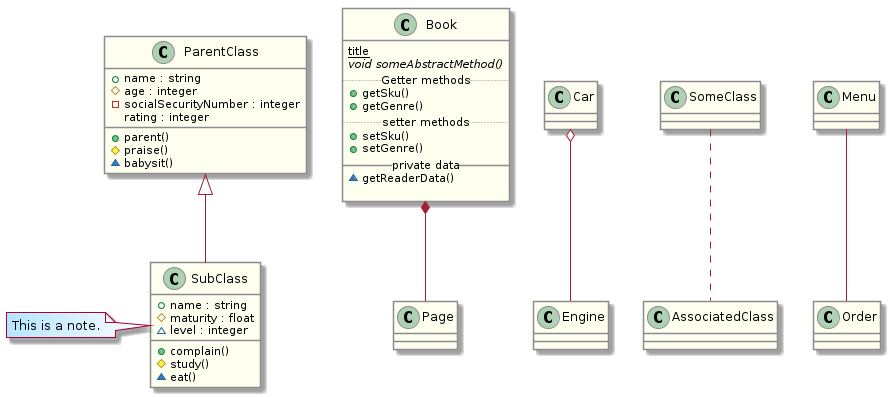
\includegraphics[width=0.70\textwidth]{class-diagram-example}}}
\caption[Class Diagram Example]{
This is a sample class diagram, see text for explanation.}
\end{figure}

\item[Component Diagram] A UML diagram that demonstrates how the modular
parts of software interact with each other using APIsi, interfaces
or other methods. The modular parts or components include databases,
web services, thin clients, thick clients, functions, libraries, and
other dependencies.

% S---------------------------------------------------------------
\item[State Diagram] A UML diagram that describes the behavior and state
of the software.
\end{description}

%
% eof
%


\pagebreak
\section{Acronyms, Commands, and Glossary}
%
% \section{Acronyms, Commands and Glossary}
%
% \acro{acronym}[short name]{full name / description}
% \ac{acronym} is the usual usage in text that defines (and gives short name)
% \acs{acronym} gives just the short name
% \acf{acronym} gives just the full name
% \acsu{acronym} gives the short name and marks it used
% \a..p{acronum} makes it plural
%
% the optional short name can include math as the acronym key cannot
% there are a zillion other options, see https://ctan.org/pkg/acronym
%
\begin{acronym}
% A---------------------------------------------------------------
\acro{A-list}{a one line description of baseline fringes used by \ac{HOPS}}
\acro{adump}{a program that dumps columns from \ac{A-list} scan data}
\acro{alist}{a program for creating a file of \ac{A-list} scan data}
\acro{aedit}{a program for editing a file of \ac{A-list} scan data}
\acro{average}{a program that calculates averages on \ac{A-list} scan data}
\acro{AIPS}{Astronomical Image Processing System}
\acro{ALMA}{Atacama Large Millimeter/Submillimeter Array}
\acro{AMP}{short for ``amplitude'' the correlation coefficient}
\acro{AP}{Acquision Period which refers to a period of time over which the
    correlator integrates the input (noisy) data to produce a usable output.
    Terms such as \acs{dump} or ``integration'' are also sometimes used,
    but both can be ambiguous.}
\acro{awk}{A programmable language for parsing line and field oriented input.
    The program was part of the original \acs{UNIX} product, and is named for
    its three authors,  Alfred Aho, Peter Weinberger, and Brian Kernighan}
% B---------------------------------------------------------------
\acro{bigendian}{refers to a computer hardware architecture where the
    most significant
    bits of a larger storage object (bytes, words\ldots) are serialized first.}
\acro{bit}{a 0 or 1}
\acro{byte}{a unit of storage corresponding to 8 bits}
% C---------------------------------------------------------------
\acro{C}{The ``C'' programming language, created to make \ac{UNIX} portable}
\acro{C++}{The C++ programming language, an object-oriented
    successor to \ac{C}}
\acro{C/C++}{Refers to code that may be either \acs{C}, \acs{C++} or a mix of
    the two ``dialects''.  The two compliers currently in use in the project,
    \acs{GCC} and \acs{Clang} manage both dialects.}
\acro{CASA}{Common Astronomy Software Applications}
\acro{channel}{an ambigous term which refers either to a spectral channel,
    \ie~frequency point of an \acsu{FFT} or to a sub-band of a
    larger receiver band.}
\acro{cofit}{a \ac{HOPS} tool to assess atmospheric coherence in terms of
    \ac{SNR} and \ac{AMP} variation with integration interval}
\acro{CorAsc2}{Correlator to Ascii (2nd version)}
\acro{cover}{a coverage test exercises all logic branches of some code module}
% D---------------------------------------------------------------
\acro{DFT}{Discrete Fourier Transform}
\acro{DR}{Delay Rate, the fringe parameter concerning
    the change of delay with time}
\acro{DiFX}{the ``distributed'' \ac{FX} correlator}
\acro{difx2mark4}{a program (part of \ac{DiFX}) to convert \ac{SWIN}
    format correlation products into the ``Mark4'' (or \acs{Mk4})
    data files used by \ac{HOPS}}
\acro{dump}{a term used with hardware correlators to refer to a time
    integration performed by hardware/firmware circuitry.  The dumped
    data may then be further integrated in software.}
% E---------------------------------------------------------------
\acro{EHT}{the Event Horizon Telescope}
\acro{EHTC}{the Event Horizon Telescope Collaboration, which usually
refers to the organization that operates the \ac{EHT}}
% F---------------------------------------------------------------
\acro{FFT}{Fast Fourier Transform}
\acro{FFTW3}{Fastest Fourier Transform in the West, version 3}
\acro{Fortran}{a FORmula TRANslation language, in common use prior to \ac{C}}
\acro{FX}{a general term for correlation that does the cross-correlation
    after first transforming to frequency space}
\acro{FITS}{Flexible Image Transport System, now referring to a
    general digital data format}
\acro{FITS-IDI}{A dialect of \ac{FITS}
    designed for the interchange of data for interferometry}
\acro{flag}{A term commonly used in radio astronomy to mark bad data
    for exclusion from further analysis.}
\acro{fourfit}{the main fringe-finding command in \ac{HOPS}}
\acro{fringex}{an \ac{HOPS} tool to explore the fringe} 
\acro{fourmer}{a program that combines data from two sub-bands into
    a larger common band}
% G---------------------------------------------------------------
\acro{ghostscript}{Ghostscript, the GNU \acs{PostScript} emulator}
\acro{Gbps}{refers to data recording rate, usually.  8 Gbps is 1 GB/s
    or one billion characters (of ASCII) per second.  Usually there
    are (packet) overheads in the actual recording so the write or
    playback speed may be somethings slightly or grossly different.
    The \ac{HOPS} era started with kbps worked through Mbps and ended
    with Gbps.  Tbps will probably be with us in another decade.}
\acro{GHz}{one billion Hz}
\acro{GNU}{GNU is Not Unix (a software project launched by
    Richard Stallman in the 80's)}
\acro{GNU/Linux}{a family of operating systems using Linus' kernel and
    GNU's software packages}
\acro{grep}{global regular expression parser, a name for a collection of
    tools that perform regular expression parsing of input data strings.}
\acro{GS}{short for \ac{ghostscript}}
\acro{GSL}{\acs{GNU} Science Library, a library of functionality for
    science applications.}
\acro{GUI}{Graphical User Interface}
% H---------------------------------------------------------------
\acro{HDF5}{Hierarchical Data Format, version 5.\protect\footnote{Why would you
    \textit{want} to use anything that took 5 versions to get right?}}
\acro{HOPS}{Haystack Observatory Postprocessing System}
\acro{Hz}{A frequency unit named for Heinrich Hertz.
    A frequency of one Hz is one oscillation per second.}
% I---------------------------------------------------------------
\acro{i/o}{short for input/output referring to the fact that programs are
    written to act on something and provide something}
\acro{IPP}{Intel Performance Primitives is a library of functionality
    optimized for use with the Intel processor family}
% J---------------------------------------------------------------
\acro{JIVE}{now just a name for an organization, it is still an
    Institution for VLBI in Europe, just not a Joint one}
% L---------------------------------------------------------------
\acro{Linux}{a family of operating systems built around Linus Torval's version
    of the UNIX kernel}
\acro{littleendian}{refers to a computer hardware architecture where the
    least significant
    bits of a larger storage object (bytes, words\ldots) are serialized first.}
\acro{LSF}{Least Squares Fit}
% M---------------------------------------------------------------
\acro{MBD}{Multi-Band Delay, the delay parameter referring to the change of
    phase with frequency in a multi-channel (sub-band) system.}
\acro{Mk4}{The fourth in a series of \ac{VLBI} hardware correlators.  The
    Mark4 replaced the Mark3 near the beginning of the millenium, and was
    finally put to rest by \ac{DiFX} in the mid 2010's}
\acro{m4py}{a shallow \acs{Python} wrapper which provides access to
    \acs{Mk4} data files and types}
\acro{MS}{Measurement Set, a formal specification for data to be analyzed
    with reference to a Measurement Equation}
\acro{MSRI}{Mid-scale Research Initiative}
% N---------------------------------------------------------------
\acro{NSF}{National Science Foundation}
\acro{ngEHT}{next-generation \acs{EHT}}
% O---------------------------------------------------------------
\acro{ovex}{an ``observer'' dialect of \acs{VEX}}
\acro{OpenMPI}{Open MPI Project is an open source Message Passing Interface
    implementation}
% P---------------------------------------------------------------
\acro{PDF}{Portable Document Format (developed by Adobe) as a successor
    to \ac{PostScript}}
\acro{PGPLOT}{a ``pretty good'' plotting package developed and maintained
    by Tim Pearson at Caltech.  He's retired now, so it is stuck at verion
    5.2.2, (released Feb 2001)}
\acro{PostScript}{a printer page description language developed by Adobe.
    \ac{fourfit} plots are currently generated in \ac{PostScript} and
    often converted to \acs{PDF}}
\acro{PERL}{Practical Extraction and Reporting Language created by Larry Wall}
\acro{PS}{short for \ac{PostScript}}
\acro{Python}{a programming language named in honor of Monty Python's Flying
    Circus}
% R---------------------------------------------------------------
\acro{RFI}{Radio Frequency Interference which is what you have when your
    receiver picks up signals you do not want}
% S---------------------------------------------------------------
\acro{SBD}{Single Band Delay, the delay parameter referring to the time
    offset between two signals being correlated}
\acro{search}{this is a tool that searches in delay/delay-rate space to
    allow visualization of a fringe peak and to aid in establishing the
    validity of more marginal-\acs{SNR} cases}
\acro{sed}{is a stream editor, that ingests line-oriented data and performs
    programmatic operations on it prior to output}
\acro{SFXC}{\acs{JIVE}'s software \ac{FX}-kind correlator}
\acro{SNR}{Signal to Noise Ratio}
\acro{SWIN}{the output format used by the \ac{DiFX} correlator}
\acro{MHO}{MIT Haystack Observatory Postprocessing System}
% T---------------------------------------------------------------
\acro{TEC}{Total Electron Content, refering to the column density of
    electrons in the line of sight through the ionosphere.  Conventionally
    one TEC Unit is \protect{$10^{16}$ electrons / m$^2$}}
% U---------------------------------------------------------------
\acro{unit}{a unit test is a short test used to validate a small part of
    some larger code module}
\acro{Unicode}{here, a general reference to a collection of methods for
    representing printable characters beyond ASCII.  The painful
    \ac{Python} 2 to 3 transition was driven by a need to more correctly
    handle strings of Unicode character representations.}
\acro{UNIX}{the name of a family of operating systems
    (born in the 70's at Bell Laboratories)}
% V---------------------------------------------------------------
\acro{VEX}{\acs{VLBI} EXperiment (file), a means of fully describing
    a planned \acs{VLBI} experiment or observation}
\acro{VEX2XML}{a program that converts \acs{VEX} files into an easily
    parsed \acs{XML} represention}
\acro{VGOS}{\acs{VLBI} Global Observing System;
    was called \acs{VLBI}2010 until the mid 2010's}
\acro{VLBI}{Very Long Baseline Interferometry}
% W---------------------------------------------------------------
\acro{Whitneys}{correlation amplitudes are normally expressed between 0 and 1,
    but in our work they are usually small and in \ac{HOPS} traditionally
    multiplied by ten thousand, in which case, the unit of correlation amplitude
    is ``Whitneys'' after Alan Whitney who may be commended or blamed for the
    usage.}
\acro{word}{an architecture-dependent unit of storage---these days, most of
    our processors use 8-\acs{byte} words}
% X---------------------------------------------------------------
\acro{XF}{a general term for correlation that does the cross-correlation
    first, and then transforms the result to frequency space}
\acro{XML}{eXtensible Markup Language}
% Z---------------------------------------------------------------
\acro{zero-pad}{the practice of extending time or frequency sequences with
    some number of zeroes which, for \ac{FFT}s has the effect of smoothing
    in the other domain}
\end{acronym} 
%
% eof
%

}

\label{page:LastPage}
\end{document}
%
% eof
%
